% Verified Mechanisms -- AAR seminar talk (MATS), 20-30 min.
% Build:  ./build.sh   (compiles, cleans aux files, publishes ../talk.pdf)
% Palette: Verified Mechanisms website, light theme (same tokens as the poster).
% Layout:  follows the thesis-defence Keynote deck (the earlier left-aligned layout
%          is kept in output/talk-old-layout/): centred titles with a short
%          rule beneath, dashed rules bracketing title/statement text, italic
%          accent-coloured subtitle, questions and captions.
\documentclass[aspectratio=169, 11pt, t]{beamer}
\usepackage[T1]{fontenc}
\usepackage[utf8]{inputenc}
\usepackage{mathpazo}
\usefonttheme{serif}
\usepackage{tikz}
\usetikzlibrary{positioning, calc, arrows.meta}
\usepackage{graphicx}
\graphicspath{{logos/}{figures/}}
\usepackage{amsmath, amssymb}

% ---- palette (verifiedmechanisms.ai, light mode) ----
\definecolor{vmnavy}{HTML}{071737}   % ink
\definecolor{vmcoral}{HTML}{C8382D}  % sharp accent
\definecolor{vmcyan}{HTML}{0B6E86}   % secondary accent / links
\definecolor{vmcream}{HTML}{FDF8EE}  % page ground
\definecolor{vmband}{HTML}{F7F1E2}   % bands
\definecolor{vmborder}{HTML}{E5DDCB} % hairlines
\definecolor{vmmuted}{HTML}{6B6F7B}  % captions, footers

\setbeamertemplate{navigation symbols}{}
\setbeamercolor{normal text}{fg=vmnavy, bg=vmcream}
\setbeamercolor{background canvas}{bg=vmcream}
\setbeamercolor{structure}{fg=vmcyan}
\setbeamercolor{frametitle}{fg=vmnavy}
\setbeamercolor{itemize item}{fg=vmcoral}
\setbeamercolor{itemize subitem}{fg=vmcoral}
\setbeamerfont{frametitle}{series=\bfseries, size={\fontsize{13.2}{16}\selectfont}}  % Georgia 21pt on the 405pt thesis page, scaled

% centred frame title with a short hairline beneath.  Geometry copied from the
% thesis deck (720x405pt): title box top 34.8pt, rule at 75.6pt, rule 50% of the
% page width, 1pt thick, accent colour at 50% opacity; scaled by 0.63 to 16:9 beamer.
\setbeamertemplate{frametitle}{%
  \nointerlineskip
  \vspace*{26.8pt}%
  % Reserve both ascender height and descender depth, including for short titles.
  {\centering\usebeamerfont{frametitle}\usebeamercolor[fg]{frametitle}\insertframetitle\vphantom{bgjpqy}\par}%
  \nointerlineskip
  \vspace*{7.7pt}%
  {\centering\color{vmcyan!50!vmcream}\rule{0.5\paperwidth}{0.63pt}\par}%
  \vspace*{2pt}%
}
\setbeamertemplate{itemize item}{\small\raisebox{0.15ex}{\usebeamercolor[fg]{itemize item}\rule{0.7ex}{0.7ex}}}
\setbeamertemplate{itemize subitem}{\footnotesize{\usebeamercolor[fg]{itemize subitem}\textbullet}}
\setbeamertemplate{footline}{%
  \hfill{\color{vmmuted}\scriptsize\insertframenumber\,/\,\inserttotalframenumber}\hspace{3mm}\vspace{1.5mm}%
}
\setbeamertemplate{caption}{\centering\small\itshape\color{vmcyan}\insertcaption\par}
% theorem-style blocks
\setbeamertemplate{blocks}[default]
\setbeamercolor{block title}{fg=vmcoral, bg=vmband}
\setbeamercolor{block body}{fg=vmnavy, bg=vmband}
\setbeamerfont{block title}{series=\bfseries, size=\small}
\setbeamerfont{block body}{size=\small}
\hypersetup{colorlinks=true, urlcolor=vmcyan, linkcolor=vmcyan}
% frame footnotes: small, grey, coral mark
\setbeamerfont{footnote}{size=\scriptsize}
\setbeamercolor{footnote}{fg=vmmuted}
\setbeamercolor{footnote mark}{fg=vmcoral}

% ---- helpers ----
\newcommand{\acc}[1]{{\color{vmcyan}#1}}
\newcommand{\pop}[1]{{\color{vmcoral}\textbf{#1}}}
\newcommand{\eyebrow}[1]{{\color{vmcoral}\bfseries\footnotesize\MakeUppercase{#1}}}
\newcommand{\muted}[1]{{\color{vmmuted}#1}}
% Keep the content below single-line subtitles at the same vertical position.
\newcommand{\slidesubtitle}[1]{\muted{\itshape #1\vphantom{bgjpqy}}\par}
\newcommand{\num}[1]{{\color{vmcoral}\bfseries\fontsize{20}{20}\selectfont #1}}
% italic accent line (questions, figure notes): \question{...}
\newcommand{\question}[1]{{\itshape\color{vmcyan}#1}}
% column label above a column: \collabel{Figure}
\newcommand{\collabel}[1]{{\footnotesize\itshape\color{vmmuted}#1}}  % thesis: 14pt on 405pt page
% dotted vertical divider between columns: \vdivider{height}
\newcommand{\vdivider}[1]{\tikz\draw[vmmuted!60, dotted, line width=0.8pt] (0,0) -- (0,#1);}
% dashed horizontal rule (the deck's signature element): \dashrule[width]
\newcommand{\dashrule}[1][11cm]{%
  \tikz[baseline=-0.5ex]\draw[vmcoral, line width=0.9pt, dash pattern=on 5pt off 3.5pt] (0,0) -- (#1,0);}
% math shorthands (as in the manuscript)
\newcommand{\hstar}{H^{\ast}}
\newcommand{\bits}{\{0,1\}}
\newcommand{\tdeg}{\deg_{\pm}}
% QR code to the blog post, top-right corner beside the centred title: \blogqr
\newcommand{\blogqr}{%
  \cornerqr{1.5cm}{qr-blog.png}{blog post}}
% QR codes to the xorformer GitHub repo and its autoresearch branch, same placement:
%   \repoqr[width]  \branchqr[width]   (width defaults to 1.5cm)
\newcommand{\cornerqr}[3]{%
  \begin{tikzpicture}[remember picture, overlay]
    \node[anchor=north east, inner sep=0pt] (cornercode)
      at ([xshift=-0.5cm, yshift=-0.35cm]current page.north east)
      {\includegraphics[width=#1]{#2}};
    \node[anchor=north, inner sep=0pt, align=center,
          font=\fontsize{6}{7}\selectfont, text=vmmuted]
      at ([yshift=-1pt]cornercode.south) {#3};
  \end{tikzpicture}}
\newcommand{\repoqr}[1][1.5cm]{\cornerqr{#1}{qr-xorformer.png}{GitHub}}
\newcommand{\branchqr}[1][1.5cm]{\cornerqr{#1}{qr-autoresearch.png}{autoresearch branch}}
% Top-anchor both boxes so large numerals align with their headings.
% numbered point: \point{1}{lead}{body}
\newcommand{\point}[3]{%
  \par\noindent\begin{minipage}[t]{0.9cm}\vspace{0pt}\num{#1}\end{minipage}%
  \begin{minipage}[t]{\dimexpr\linewidth-0.9cm\relax}\raggedright
    \vspace{0pt}{\bfseries #2}\\[0.05cm]{\color{vmnavy!85}#3}\end{minipage}\par}
% full-slide statement between dashed rules: \statement[subtitle]{text}
% (placed with a page overlay: beamer's [c] option leaves the block above centre)
% footnote for a statement slide, placed by hand at the height of the regular-slide
% footnotes (a plain frame has no footline, so Beamer would drop it to the page edge)
\newcommand{\statementfn}[1]{%
  \begin{tikzpicture}[remember picture, overlay]
    \node[anchor=south west, text width=0.85\paperwidth, font=\scriptsize, text=vmmuted,
          inner sep=0pt] (sfn) at ([xshift=1.0cm, yshift=0.6cm]current page.south west)
      {\textsuperscript{\color{vmcoral}\thefootnote}#1};
    \draw[vmnavy, line width=0.4pt] ([yshift=3pt]sfn.north west) -- ++(3.6cm,0);
  \end{tikzpicture}}
\newcommand{\statementfootnote}{}
\newcommand{\statement}[2][]{%
  \begin{frame}[plain]
    \begin{tikzpicture}[remember picture, overlay,
        every node/.style={inner sep=0pt, outer sep=0pt}]
      \def\stmtsub{#1}%
      \node[anchor=center, text width=13.5cm, align=center] (stmt) at (current page.center)
        {{\fontsize{24}{30}\selectfont\color{vmnavy} #2\par}%
         \ifx\stmtsub\empty\else
           \vspace{0.35cm}%
           \noindent\hspace*{\fill}\parbox{11cm}{\centering
             \fontsize{13}{16.5}\selectfont\itshape\color{vmnavy!85} #1\par}\hspace*{\fill}\par
         \fi};
      \coordinate (l) at ([xshift=-5.6cm]current page.center);
      \coordinate (r) at ([xshift=5.6cm]current page.center);
      \coordinate (t) at ([yshift=0.5cm]stmt.north);
      \coordinate (b) at ([yshift=-0.5cm]stmt.south);
      \draw[vmcoral, line width=0.9pt, dash pattern=on 5pt off 3.5pt] (l |- t) -- (r |- t);
      \draw[vmcoral, line width=0.9pt, dash pattern=on 5pt off 3.5pt] (l |- b) -- (r |- b);
    \end{tikzpicture}
    % optional footnote: \gdef\statementfootnote{\statementfn{text}} before the call and
    % \footnotemark in the text; cleared after use
    \statementfootnote\gdef\statementfootnote{}%
  \end{frame}}

\begin{document}

% =====================================================================
% 1. Title
% =====================================================================
\begin{frame}[plain]
  \begin{tikzpicture}[remember picture, overlay,
      every node/.style={inner sep=0pt, outer sep=0pt}]
    \coordinate (n)  at (current page.north);
    \coordinate (sw) at (current page.south west);
    \coordinate (se) at (current page.south east);

    % title block between dashed rules
    \draw[vmcoral, line width=0.9pt, dash pattern=on 5pt off 3.5pt]
      ([xshift=-5.6cm, yshift=-1.75cm]n) -- ([xshift=5.6cm, yshift=-1.75cm]n);
    \node[anchor=north, text width=14cm, align=center] at ([yshift=-2.3cm]n)
      {\fontsize{34}{38}\selectfont\color{vmnavy} Verified Mechanisms\par};
    \node[anchor=north, text width=14cm, align=center] at ([yshift=-3.75cm]n)
      {\fontsize{16.5}{20.5}\selectfont\color{vmnavy!85}%
       Formally verified autoresearch\\for theoretical mech interp\par};
    \draw[vmcoral, line width=0.9pt, dash pattern=on 5pt off 3.5pt]
      ([xshift=-5.6cm, yshift=-5.45cm]n) -- ([xshift=5.6cm, yshift=-5.45cm]n);

    % author block
    \node[anchor=north, text width=14cm, align=center] at ([yshift=-5.95cm]n)
      {{\large\color{vmnavy} Karthik Viswanathan}\\[0.18cm]
       \muted{\small MATS 9.1}\\[0.1cm]
       \muted{\small Automated Alignment Research Seminar, September 2026}\par};

    % footer: VM logo (left), site (centre), MATS (right)
    \node[anchor=west] at ([xshift=1.1cm, yshift=0.75cm]sw)
      {
\includegraphics[height=0.95cm]{vm-logo-light-bg.pdf}};
    \node[anchor=center] at ([yshift=0.75cm]sw-|current page.center)
      {\muted{\footnotesize\texttt{verifiedmechanisms.ai}}};
    \node[anchor=east] at ([xshift=-1.1cm, yshift=0.75cm]se)
      {
\includegraphics[height=0.55cm]{mats_navy.png}};
  \end{tikzpicture}
\end{frame}

% =====================================================================
% 2. About me
% =====================================================================
\begin{frame}{About me}
  \vspace{0.1cm}
  \begin{columns}[T, totalwidth=\textwidth]
    \begin{column}{0.5\textwidth}
      \point{1}{Now: Simplex (MATS 9.1)}
        {\fontsize{9}{10.8}\selectfont How does post-training reshape the internal mechanisms? ft.\ modular~addition\par}

      \vspace{0.50cm}
      \point{2}{Before: Geodesic (MARS 3.0)}
        {\fontsize{9}{10.8}\selectfont A transformer architecture alteration to incentivise externalised reasoning \par}


      \vspace{0.5cm}
      \point{3}{Research taste}
        {\fontsize{9}{10.8}\selectfont I end up working on the full range of models, from toy examples to models at scale.\par}

      % \vspace{0.55cm}
      % \point{3}{Opinion}
      %   {I think interpretability-informed control is hard, but would be cool if it works out.}
    \end{column}

    \begin{column}{0.48\textwidth}
      \centering
      % hand-drawn cartoon; the TikZ version lives in figures/about-me-cartoon.tex
      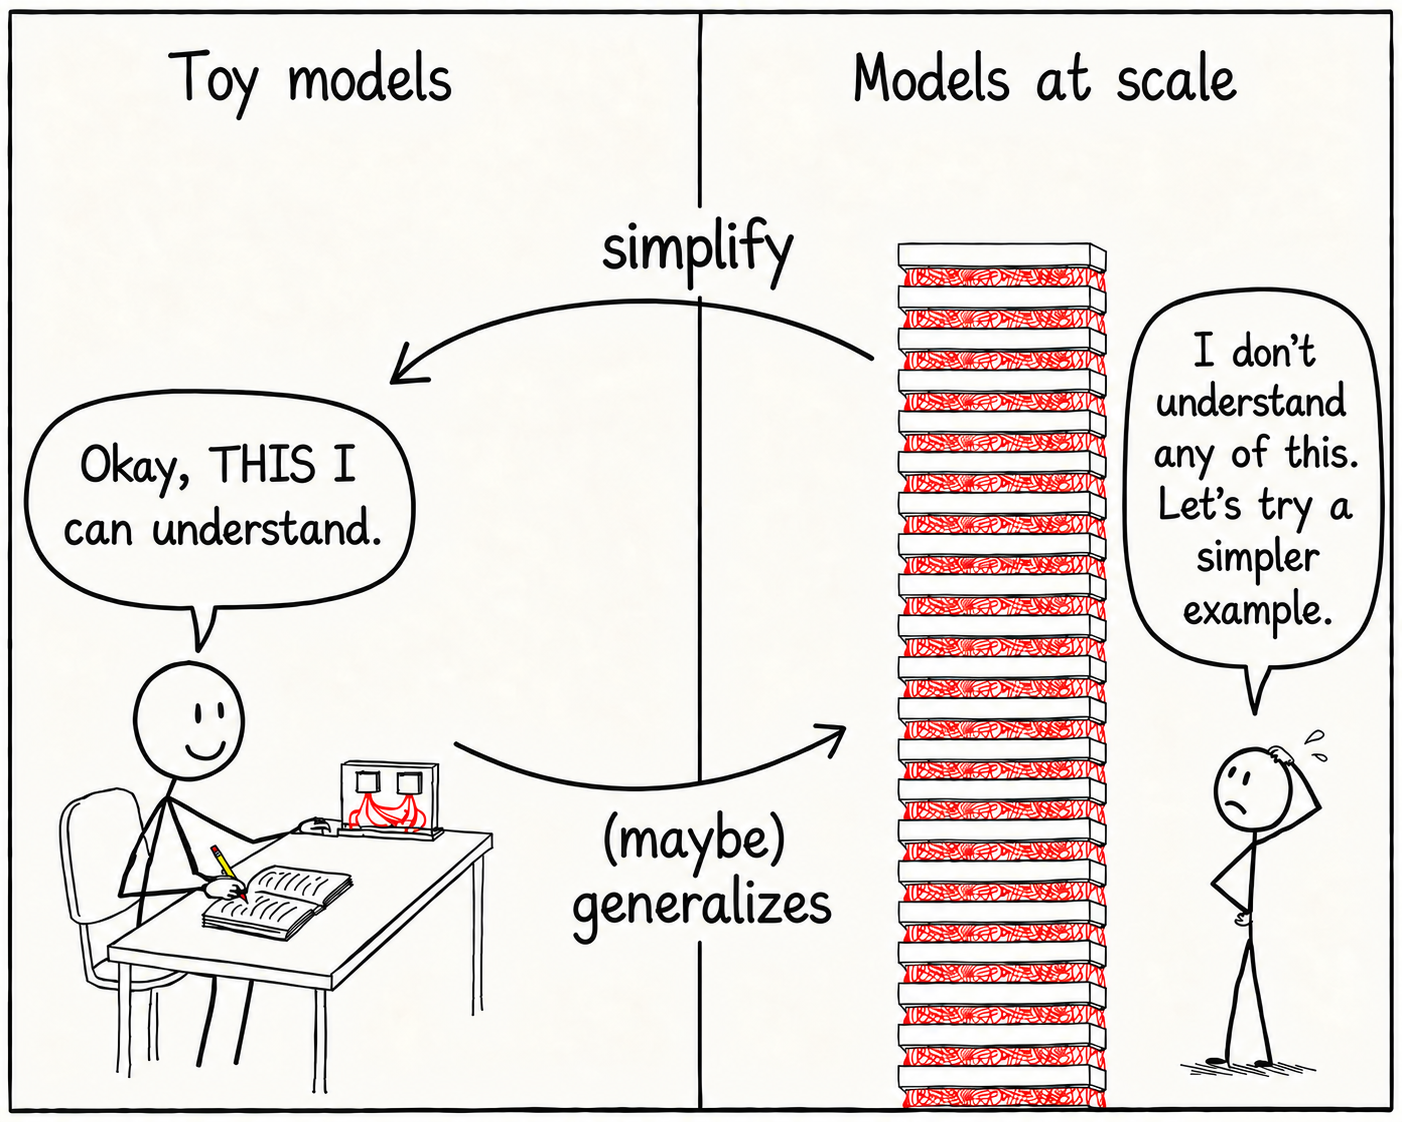
\includegraphics[width=\linewidth]{toy-models-vs-models-at-scale.png}
    \end{column}
  \end{columns}
\end{frame}

% =====================================================================
% 3. Hook
% =====================================================================
\statement[A minimal proof of concept showing how formally verified autoresearch can help mech interp researchers.]{To introduce Verified Mechanisms, let me begin with a short story.}

% =====================================================================
% 4. The origin story
% =====================================================================
\begin{frame}{The origin story}
  \vspace{-0.1cm}
  \centering
  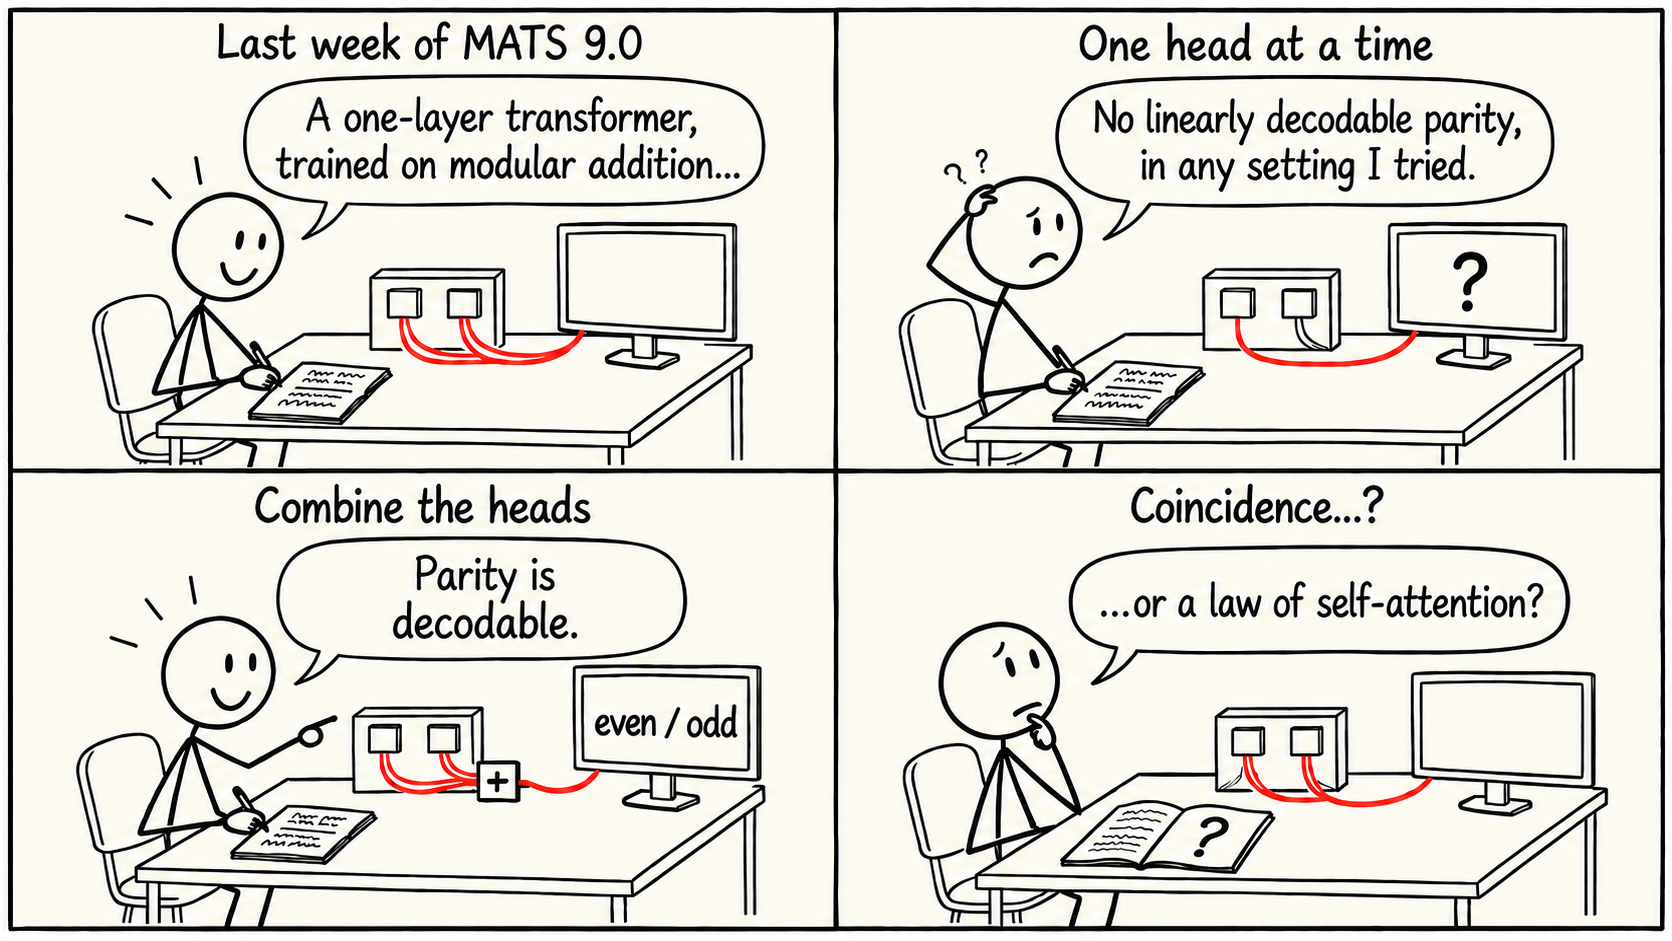
\includegraphics[height=6.1cm]{slide4-parity-decoding-cartoon.png}
\end{frame}

% =====================================================================
% 5. In search of a law of self-attention
% =====================================================================
\begin{frame}{In search of a ``law of self-attention''}
  \vspace{-0.3cm}
  \centering
  {\large\question{``Can an attention head compute XOR?''}\par}

  \vspace{0.3cm}
  \begin{columns}[T, totalwidth=\textwidth]
    \begin{column}{0.52\textwidth}
      \small
      \point{1}{Ask frontier models}
        {While out on a walk, I posed the question to Opus~4.7 and GPT-5.4.}

      \vspace{0.3cm}
      \point{2}{One hour later}
        {Both returned (fairly involved) answers.\footnotemark}

      \vspace{0.3cm}
      \point{3}{Formalise the proof}
        {I asked Opus to formalise GPT's argument in Lean~4, and the proof checked out!}
    \end{column}
    \begin{column}{0.46\textwidth}
      \centering
      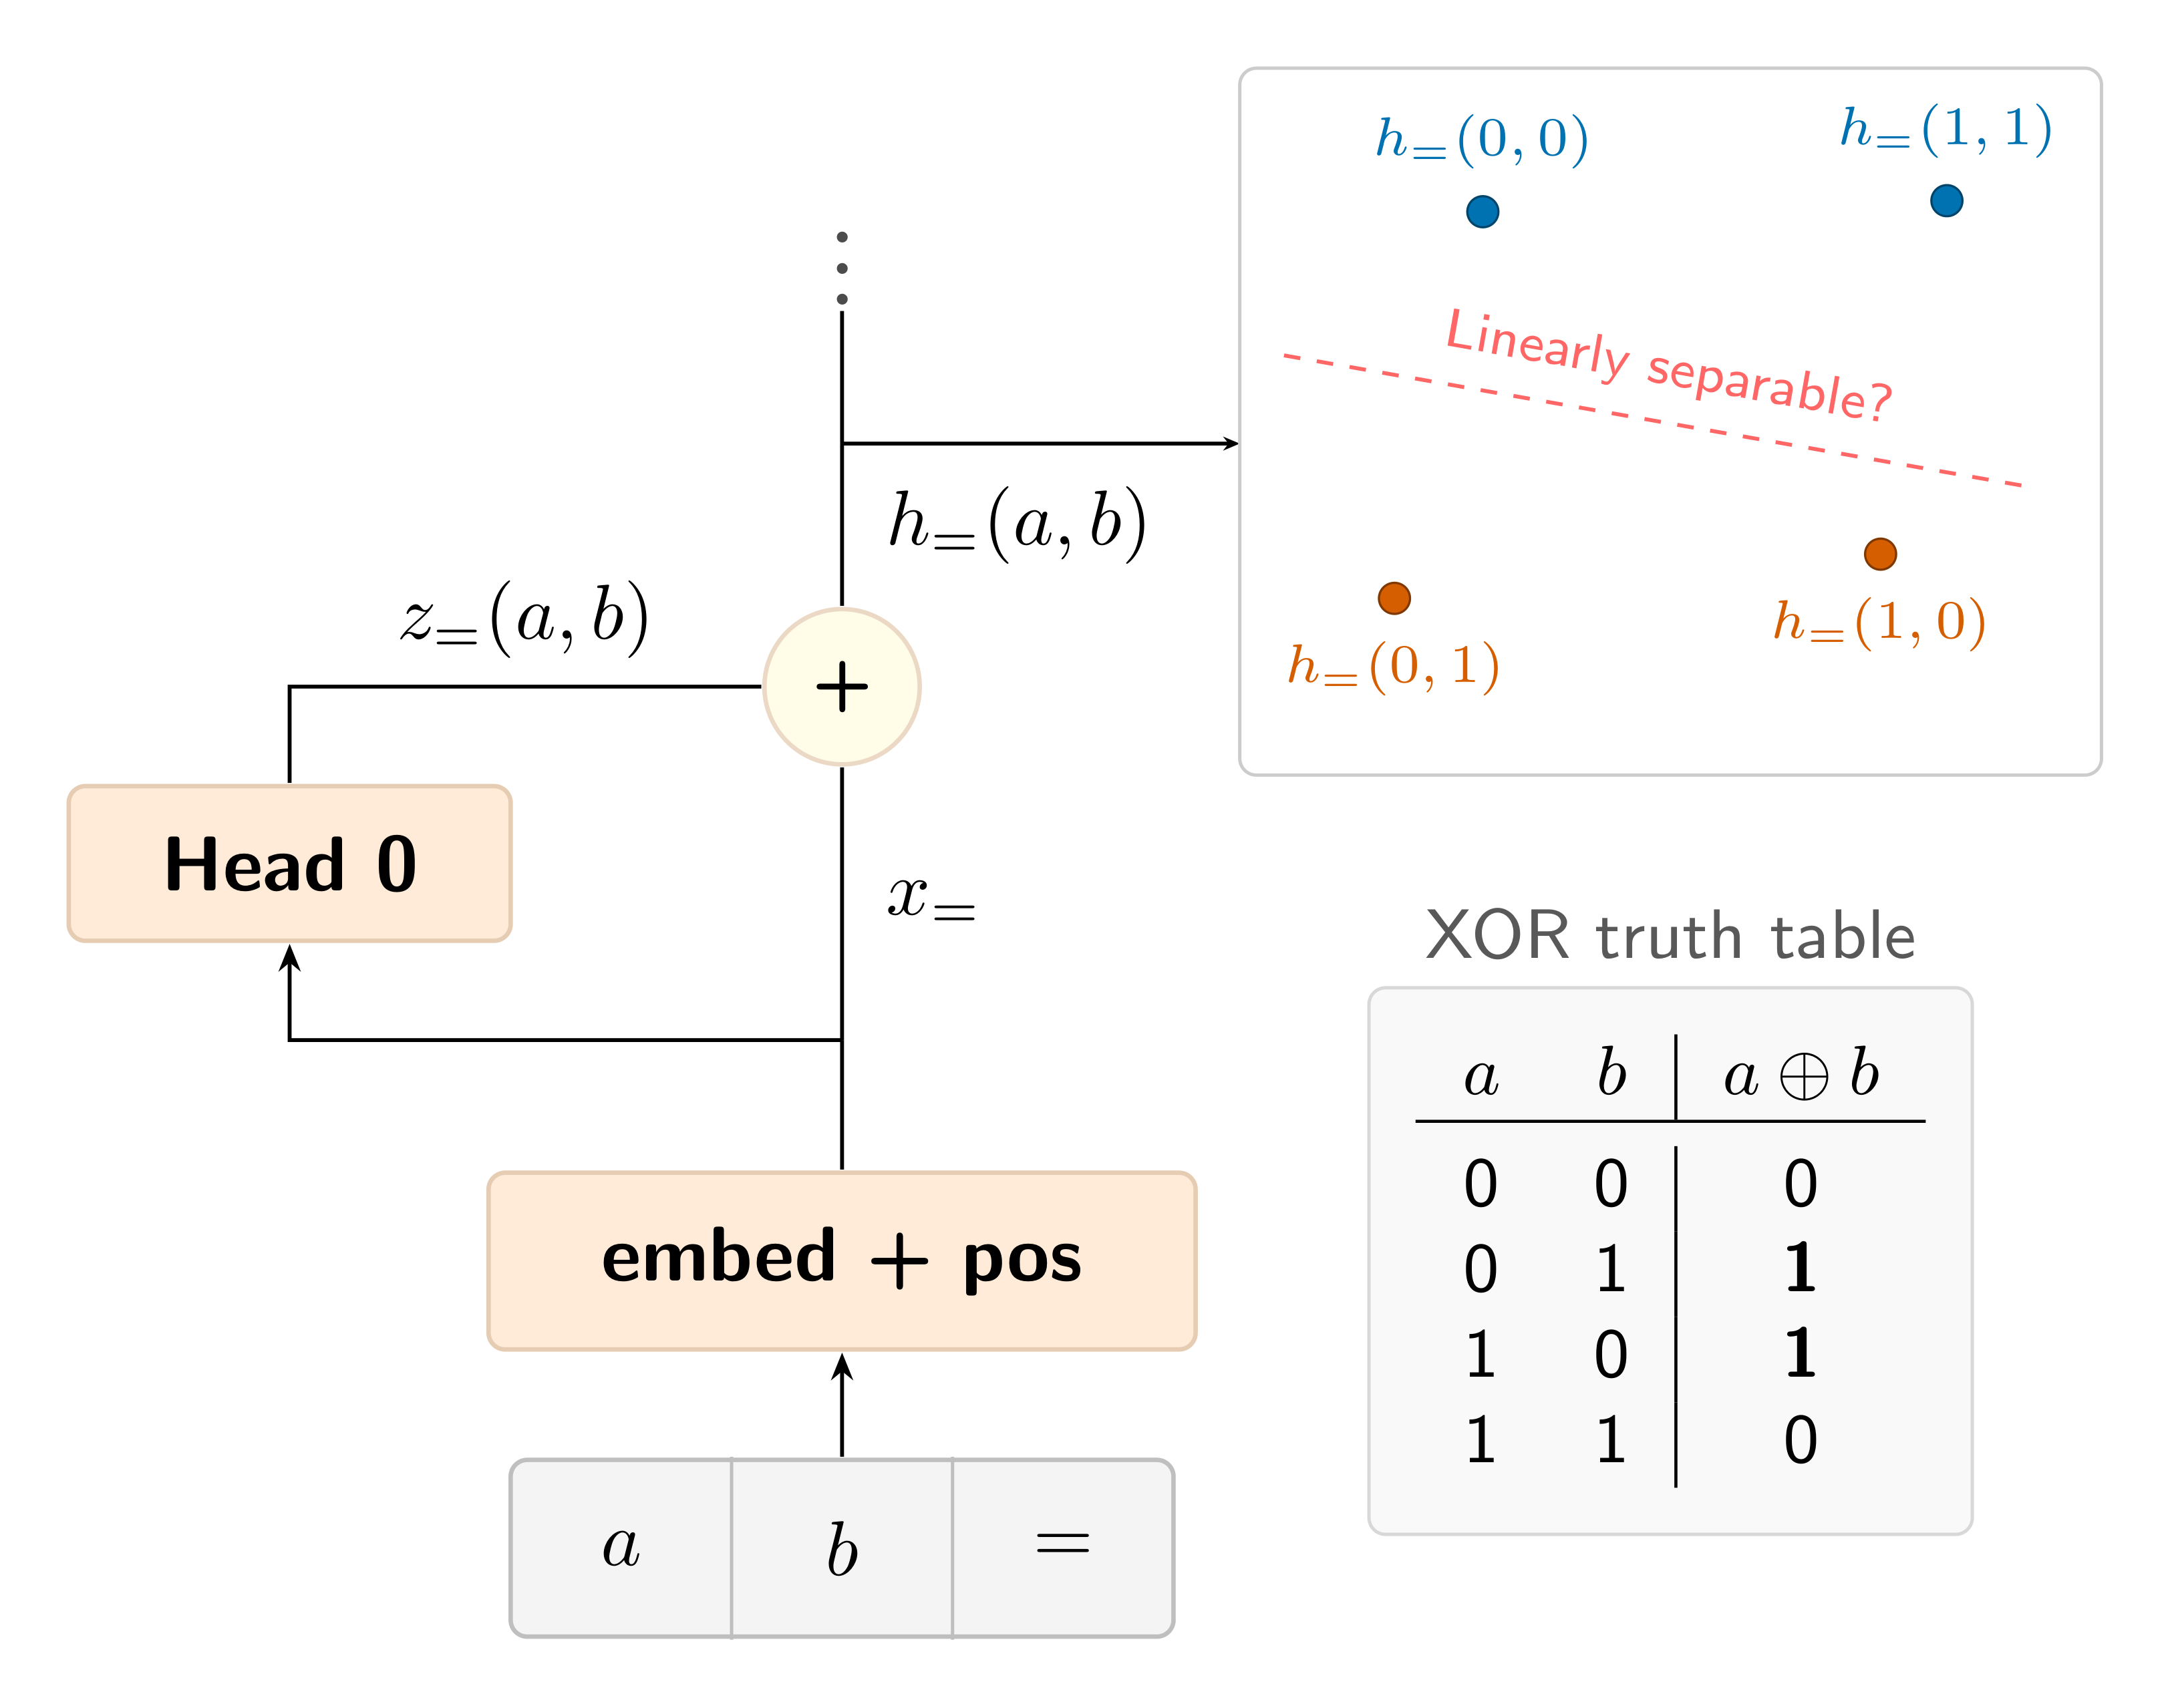
\includegraphics[width=0.88\linewidth]{xor-architecture.png}

      \vspace{0.05cm}
      {\scriptsize\question{Linearly separable into XOR classes?}\par}
    \end{column}
  \end{columns}
  % footnote text sits outside the \point minipage so it lands at the frame bottom
  \footnotetext{Opus' argument even contained a couple of hallucinated steps.}
  \blogqr
\end{frame}

% =====================================================================
% 6. First law of self-attention
% =====================================================================
\begin{frame}{Outcome: first law of self-attention}
  \vspace{0.5cm}
  % [T]: the block (right) shares its top edge with the figure panel (left); their heights match
  \begin{columns}[T, totalwidth=\textwidth]
    \begin{column}{0.5\textwidth}
      \centering
      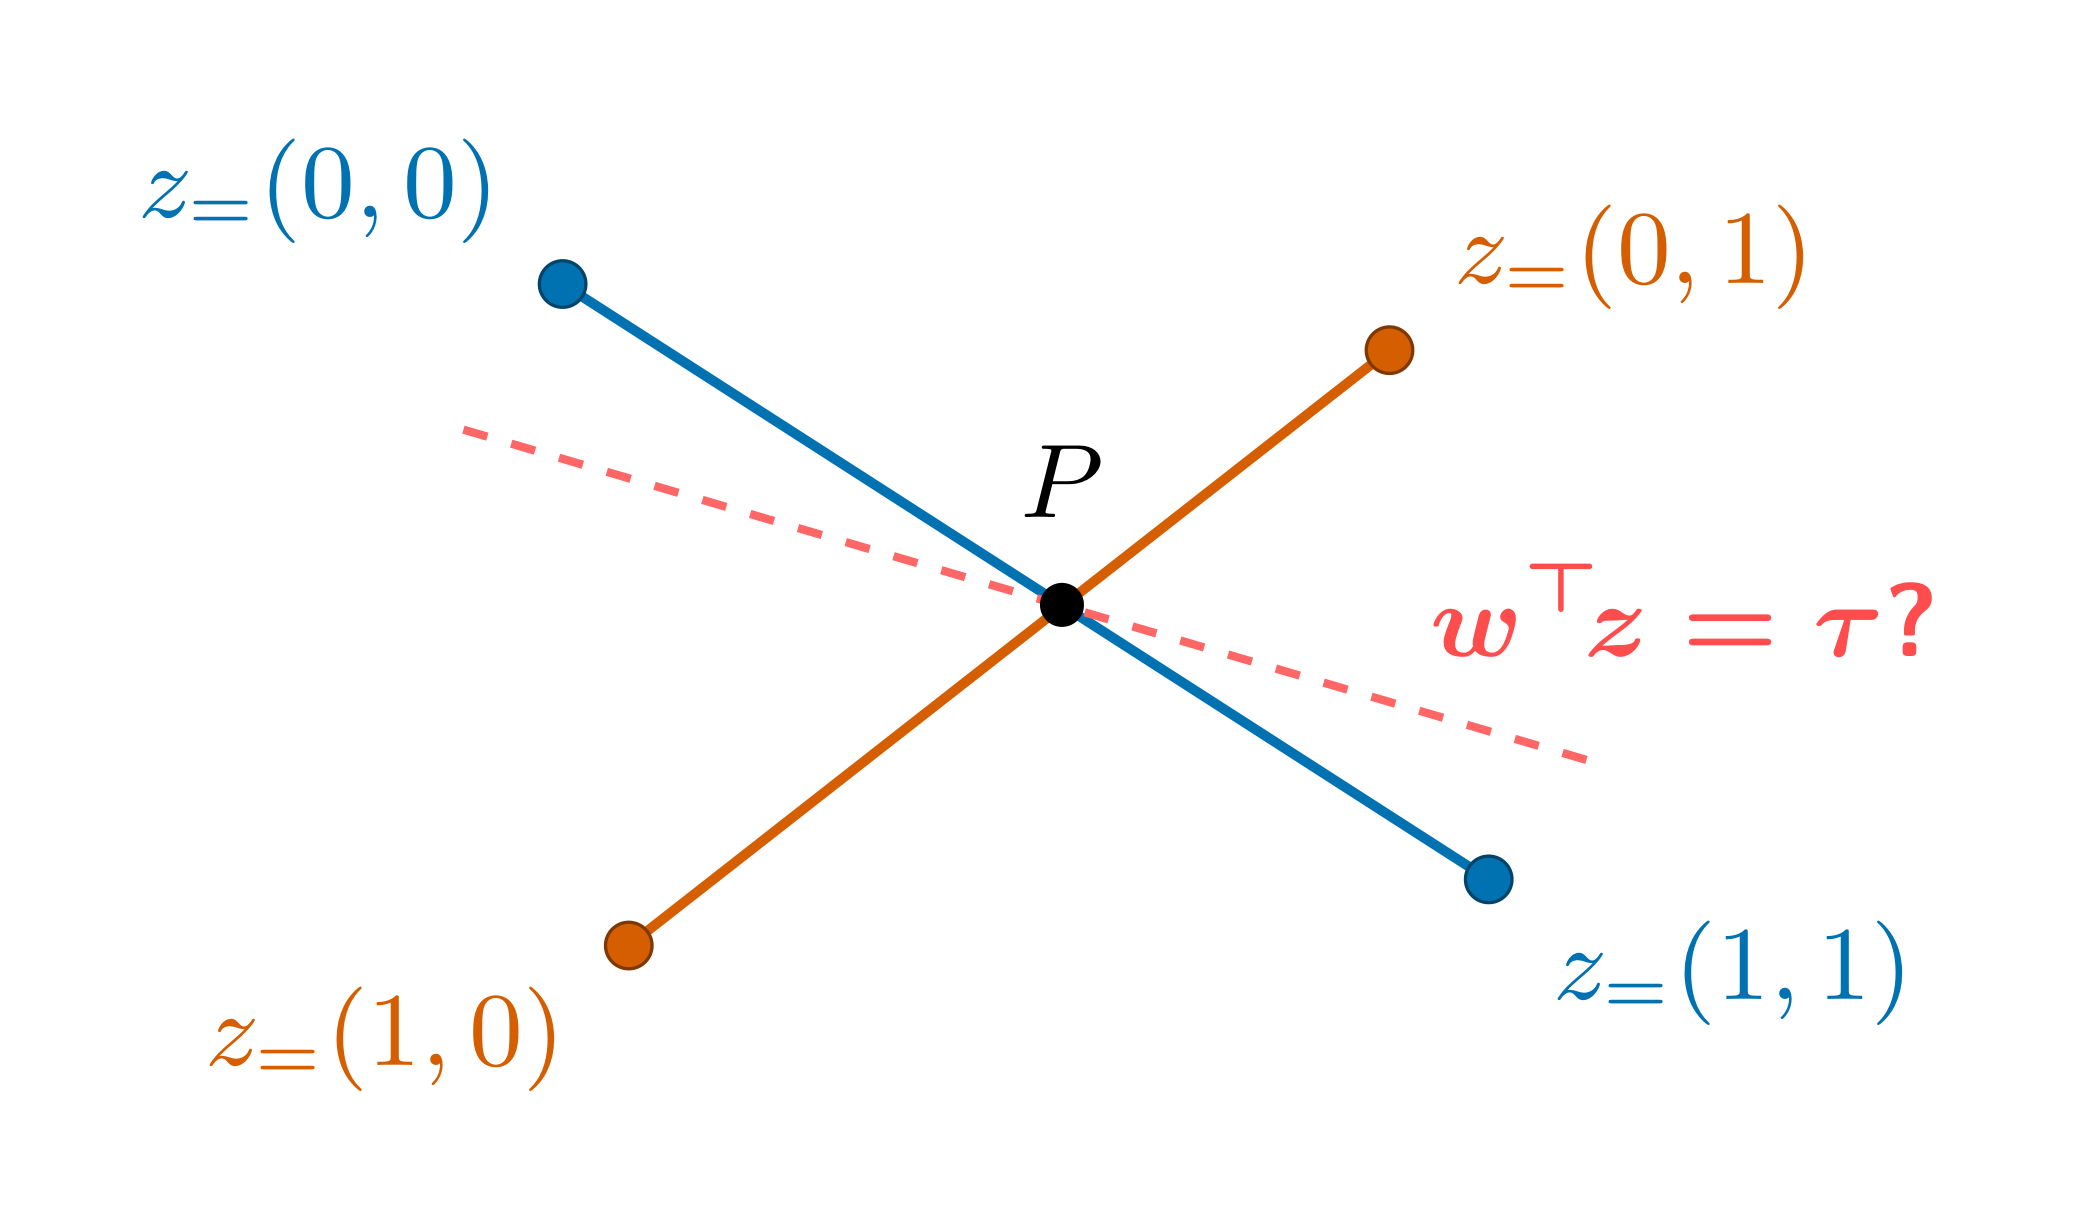
\includegraphics[width=\linewidth]{xor-geometry-left.png}

      \vspace{0.05cm}
      {\scriptsize\muted{Attention outputs $z_=(a,b)$ for the four inputs:\\ blue for even parity, orange for odd parity.}\par}
    \end{column}
    \begin{column}{0.46\textwidth}
      \vspace{-\medskipamount}% cancel the skip Beamer puts above a block
      \begin{block}{}
        \pop{One head cannot compute XOR.}

        %\vspace{0.1cm}
        \muted{\footnotesize ft. a surprisingly elegant proof by GPT-5.4, formalised by~Opus~4.7.}

        \vspace{0.3cm}
        After a single attention-head update, the line segment joining the even-parity outputs always intersects the segment joining the odd-parity outputs, ruling out their linear separability. 

        % \vspace{0.3cm}
        % Therefore, a single attention head cannot linearly separate the two classes.

      \end{block}

      % \vspace{0.3cm}
      % \small
      % The segment $[z_=(0,0),\,z_=(1,1)]$ crosses $[z_=(0,1),\,z_=(1,0)]$ at a point $P$,
      % so no hyperplane $w^{\top}z=\tau$ separates the two classes.
    \end{column}
  \end{columns}
  \blogqr
\end{frame}

% =====================================================================
% 7. A simple question hides a difficult proof
% =====================================================================
\begin{frame}{Questions are easy, proofs are hard}
  \vspace{-0.3cm}
  \centering
  \slidesubtitle{At least, they used to be.}

  \vspace{0.4cm}
  % labels on their own row so they share a baseline
  \begin{columns}[T, totalwidth=\textwidth]
    \begin{column}{0.30\textwidth}
      \centering{\small\bfseries\color{vmnavy}What I wanted to know}\par
    \end{column}
    \begin{column}{0.04\textwidth}
      % top anchor for the divider drawn after the columns
      \centering\tikz[remember picture, overlay]\coordinate (divtop);\par
    \end{column}
    \begin{column}{0.64\textwidth}
      \centering{\small\bfseries\color{vmnavy}What I would need to analyse}\par
    \end{column}
  \end{columns}

  \vspace{0.55cm}
  % content row: question and formulas centred against each other
  \begin{columns}[c, totalwidth=\textwidth]
    \begin{column}{0.30\textwidth}
      \centering
      {\Large\pop{``Can an attention head compute XOR?''}\par}
    \end{column}
    \begin{column}{0.04\textwidth}\end{column}
    \begin{column}{0.64\textwidth}
      \centering
      {\Large $\displaystyle
        h_=(a,b) = x_= + z_=(a,b)
      $\par}

      \vspace{0.65cm}
      \resizebox{\linewidth}{!}{$\displaystyle
        z_=(a,b)=
        \frac{\sum_{j\in\{a,b,=\}}\exp\!\bigl(x_=^{\top} W_Q^{\top} W_K\, x_j\bigr)\,W_V\, x_j}
             {\sum_{j\in\{a,b,=\}}\exp\!\bigl(x_=^{\top} W_Q^{\top} W_K\, x_j\bigr)}
      $}\tikz[remember picture, overlay]\coordinate (divbot);\par
    \end{column}
  \end{columns}
  % dotted divider spanning the labels and the formulas
  \begin{tikzpicture}[remember picture, overlay]
    \coordinate (divend) at (divtop |- divbot);
    \draw[vmmuted!60, dotted, line width=0.8pt]
      ([yshift=0.3cm]divtop) -- ([yshift=-0.8cm]divend);
  \end{tikzpicture}

  \vspace{0.55cm}
  \centering
  {\large\question{The cost of pursuing hard mathematical questions is lower now,\\ thanks to formally verified autoresearch.}\par}
\end{frame}

% =====================================================================
% 8. More laws of self-attention
% =====================================================================
\begin{frame}{Slightly scaling up: more laws of self-attention}
  \vspace{-0.3cm}
  \centering
  \slidesubtitle{Longer runs: GPT-5.5 conjectures and proves, Claude 4.8 formalises in Lean~4.}

  \vspace{0.25cm}
  \begin{minipage}{0.92\textwidth}
    \small
    \begin{block}{The pilot problem}
      How many heads does it take to represent a Boolean function $f:\bits^n\to\bits$?\par
      \vspace{0.12cm}
      {\centering $\hstar(f)=\min\{H:\ f\text{ is representable by an $H$-head model}\}.$\par}
      \vspace{0.12cm}
      % the fewest attention heads for which one attention update makes the inputs with
      % $f=0$ and $f=1$ linearly separable at the readout position.
    \end{block}

    \vspace{0.2cm}
    \begin{block}{Theorem (symmetric functions)}
      A closed form for $\hstar(f)$ for every symmetric Boolean function, $\hstar(f) = C(f)$.\footnotemark \\[0.25cm]
      \pop{Corollary:} $\hstar(\text{XOR}_n) = n$.
    \end{block}
  \end{minipage}
  % footnote text outside the minipage so it lands at the frame bottom
  \footnotetext{The proof is left as an exercise for the reader and their LLM.}
  \repoqr
\end{frame}

% =====================================================================
% 9. The big picture
% =====================================================================
% \begin{frame}{The big picture}
%   \vspace{-0.05cm}
%   \centering
%   % audience version; the literal redraw of the SVG is figures/big-picture.tex
%   \input{figures/big-picture-friendly.tex}

%   \vspace{0.05cm}
%   {\small\question{From research questions to formally verified results}}
% \end{frame}

% =====================================================================
% Zooming out (section statement before the big picture and impact)
% =====================================================================
\statement[From pilot question to research programme]{Zooming out.}

% =====================================================================
% 10. What is Verified Mechanisms?
% =====================================================================
\begin{frame}{What is Verified Mechanisms?}
  % Points are verbatim from the Manifund proposal's project summary
  % (xorformer/writeup/helper-docs/proposal.md).
  \vspace{-0.3cm}
  \centering
  \slidesubtitle{Formally verified autoresearch for theoretical mech interp}

  \vspace{0.5cm}
  \begin{columns}[T, totalwidth=\textwidth]
    \begin{column}{0.58\textwidth}
      \small
      \point{1}{Goal}
        {We aim to produce foundational results in mechanistic interpretability by leveraging the recent advances in the mathematical abilities of frontier~models.}

      \vspace{0.5cm}
      \point{2}{Verification}
        {To make sure that the theorems provided by the frontier models do not contain logical flaws, we formally verify them in Lean~4.}

      % \vspace{0.5cm}
      % \point{3}{Ambition}
      %   {Preliminary analyses hint at a mathematical abstraction (imagine Feynman diagrams) for multihead attention to advance foundational mech interp.}
    \end{column}
    \begin{column}{0.38\textwidth}
      \centering
      \vspace{0.45cm}
      
\includegraphics[width=0.62\linewidth]{vm-logo-light-bg.pdf}

      \vspace{0.3cm}
      {\muted{\footnotesize\texttt{verifiedmechanisms.ai}}\par}
    \end{column}
  \end{columns}
\end{frame}

% =====================================================================
% 11. What is Verified Mechanisms? (reveal: where the logo comes from)
% =====================================================================
\begin{frame}{What is Verified Mechanisms?}
  % reveal: same slide, the logo's inspiration in place of the logo
  % Points are verbatim from the Manifund proposal's project summary
  % (xorformer/writeup/helper-docs/proposal.md).
  \vspace{-0.3cm}
  \centering
  \slidesubtitle{Formally verified autoresearch for theoretical mech interp}

  \vspace{0.5cm}
  \begin{columns}[T, totalwidth=\textwidth]
    \begin{column}{0.58\textwidth}
      \small
      \point{1}{Goal}
        {We aim to produce foundational results in mechanistic interpretability by leveraging the recent advances in the mathematical abilities of frontier~models.}

      \vspace{0.5cm}
      \point{2}{Verification}
        {To make sure that the theorems provided by the frontier models do not contain logical flaws, we formally verify them in Lean~4.}

      % \vspace{0.5cm}
      % \point{3}{Ambition}
      %   {Preliminary analyses hint at a mathematical abstraction (imagine Feynman diagrams) for multihead attention to advance foundational mech interp.}
    \end{column}
    \begin{column}{0.38\textwidth}
      \centering
      \vspace{0.45cm}
      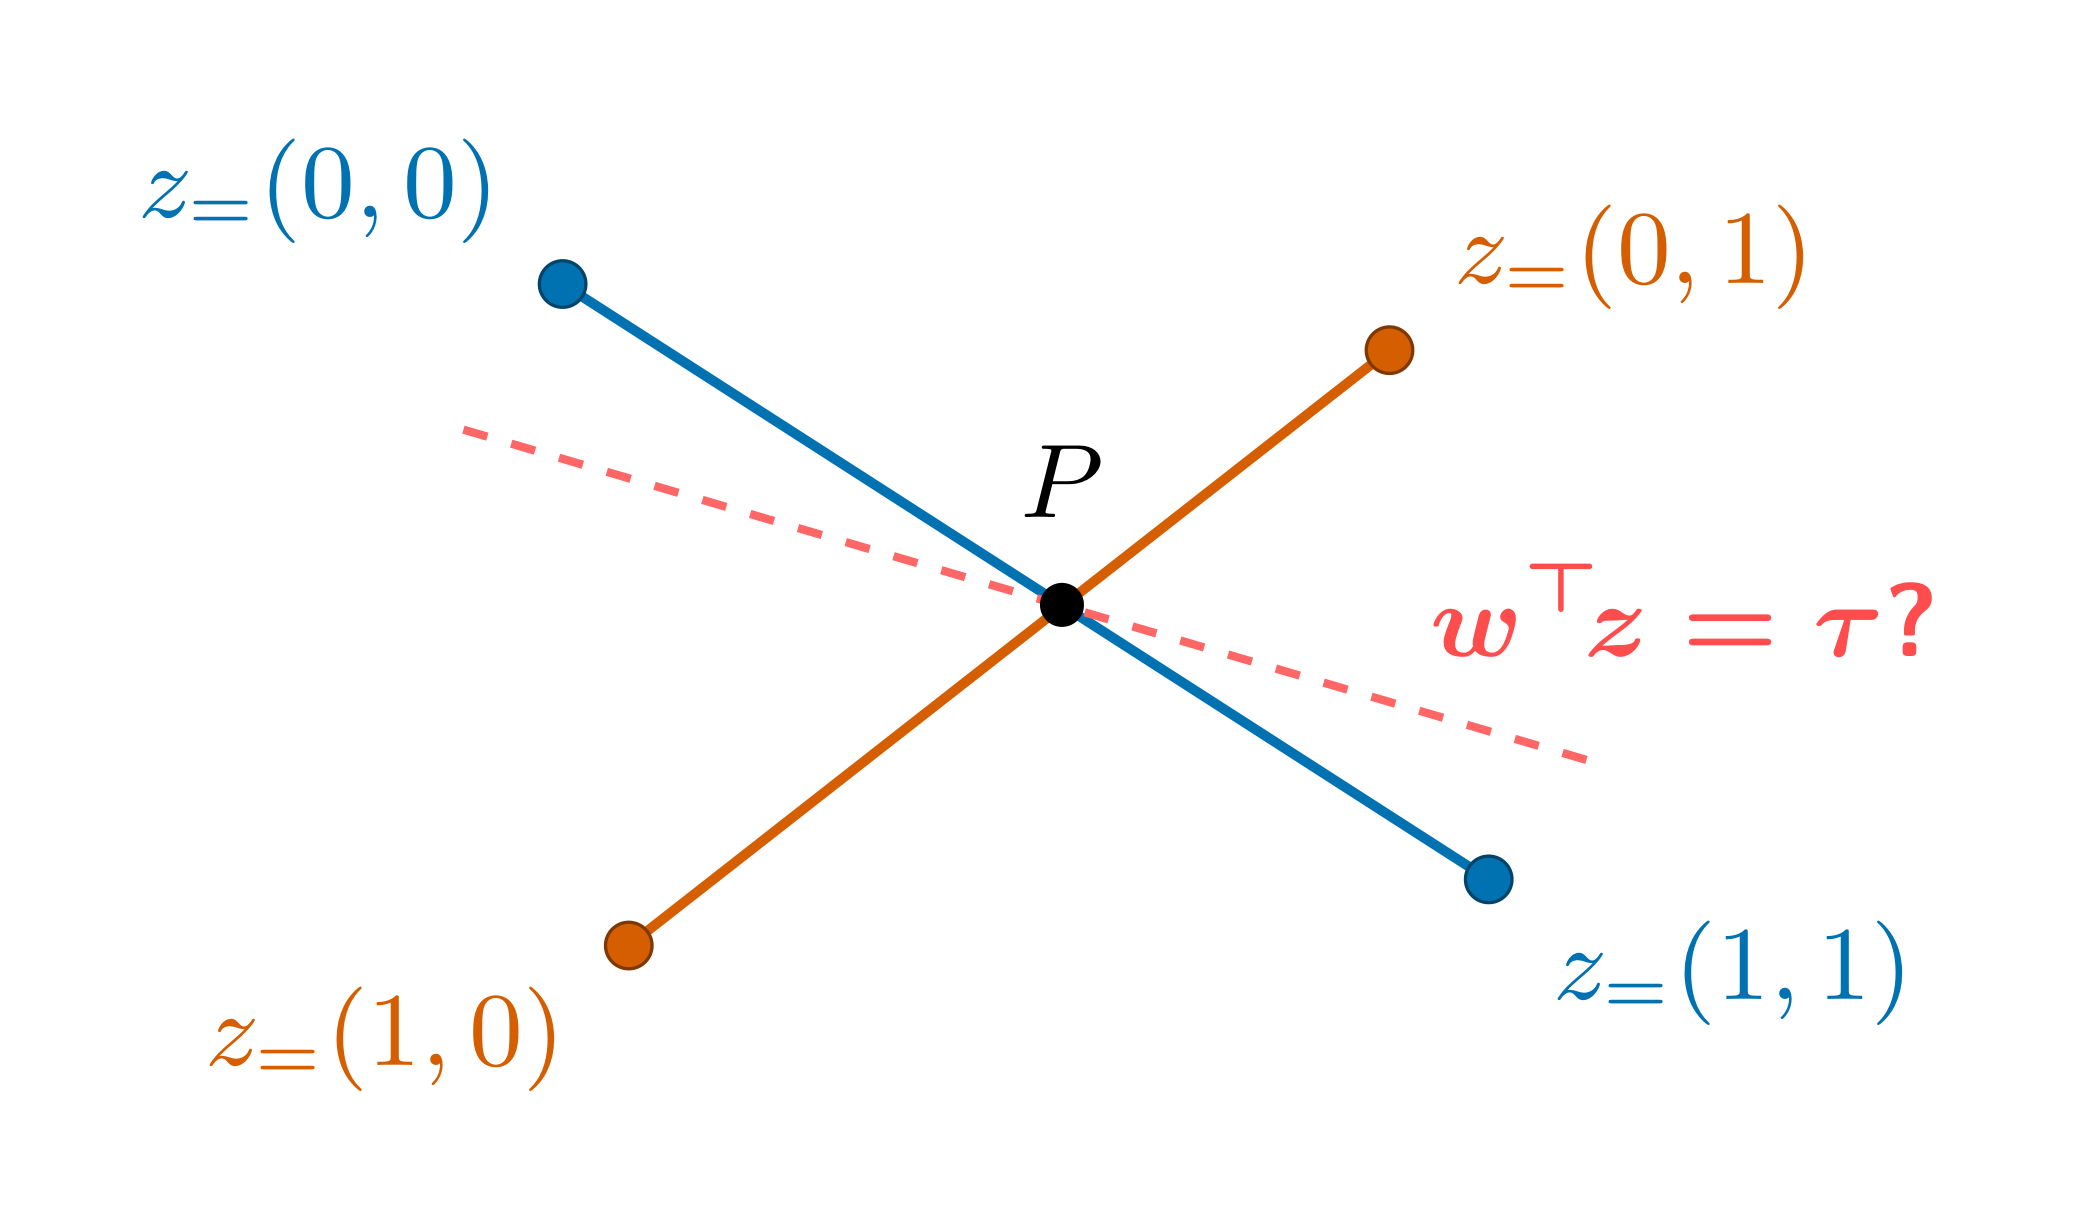
\includegraphics[width=\linewidth]{xor-geometry-left.png}

      \vspace{0.3cm}
      {\muted{\footnotesize First law of self-attention}\par}
    \end{column}
  \end{columns}
\end{frame}

% =====================================================================
% 12. Impact
% =====================================================================
\begin{frame}{Theory of impact}
  % Every sentence below is verbatim from the Manifund proposal (xorformer/writeup/helper-docs/proposal.md).
  \vspace{-0.3cm}
  \centering
  \slidesubtitle{Why should we do theoretical mech interp?}

  \vspace{0.3cm}
  \begin{columns}[T, totalwidth=\textwidth]
    \begin{column}{0.47\textwidth}
      \centering
      {\small\itshape\color{vmmuted}Precedent}\par
      \vspace{0.3cm}
      \begin{minipage}{0.95\linewidth}\small\raggedright
        \pop{Foundational theory has shaped mechanistic~interpretability before.}\\[0.2cm]
        Elhage et~al.\ (2021) worked out the
        mathematics of attention from first principles, and many later mechanistic interpretability
        ideas (for example, induction heads, transformer circuits) build on that~framework.
      \end{minipage}
    \end{column}
    \begin{column}{0.04\textwidth}
      \centering
      \vdivider{4.2cm}
    \end{column}
    \begin{column}{0.47\textwidth}
      \centering
      {\small\itshape\color{vmmuted}Our contribution}\par
      \vspace{0.3cm}
      \begin{minipage}{0.95\linewidth}\small\raggedright
        \pop{Our aim is more modest than Elhage et~al.\ but similar in~spirit.}\\[0.2cm]
        A growing library of machine-checked theorems that applied researchers can use as reference
        points, and a workflow for producing them faster than hand-derivation alone.
      \end{minipage}
    \end{column}
  \end{columns}
\end{frame}

% =====================================================================
% 13. Why formally verified autoresearch?
% =====================================================================
\begin{frame}{Why formally verified autoresearch for theoretical mech interp?}
  % Every sentence below is verbatim from the Manifund proposal (02-manuscript/writeup-proposal.md).
  \vspace{0.55cm}
  \begin{columns}[T, totalwidth=\textwidth]
    \begin{column}{0.47\textwidth}
      \centering
      {\small\itshape\color{vmmuted}Need for autoresearch}\par
      \vspace{0.3cm}
      \begin{minipage}{0.95\linewidth}\small\raggedright
        \pop{Foundational theory is hard to scale with human effort alone.}\\[0.2cm]
        Hand-derivation is slow and expertise-intensive, and frontier models can now carry much of this load.
      \end{minipage}
    \end{column}
    \begin{column}{0.04\textwidth}
      \centering
      \vdivider{3.4cm}
    \end{column}
    \begin{column}{0.47\textwidth}
      \centering
      {\small\itshape\color{vmmuted}Need for formal verification}\par
      \vspace{0.3cm}
      \begin{minipage}{0.95\linewidth}\small\raggedright
        \pop{Unverified autoresearch can fail~quietly.}\\[0.2cm]
    Long derivations by frontier models can hide subtle errors that human review could miss.
    Lean checks every step and rejects invalid proofs.
      \end{minipage}
    \end{column}
  \end{columns}
\end{frame}

% =====================================================================
% 14. More concretely, how we hope to contribute
% =====================================================================
\begin{frame}{More concretely, how we hope to contribute}
  % Bodies adapted from the AutoMLR submission (02-manuscript/neurips_2026.tex, Introduction
  % and Significance), generalised from attention heads to transformer components.
  \vspace{0.78cm}
  \centering
  \begin{minipage}{0.92\textwidth}
    \small
    \point{1}{Stronger fundamentals for toy-model research}
      {Foundational theory of transformer components can provide a principled basis for
       interpreting and generalising empirical findings from toy models.}

    \vspace{0.5cm}
    \point{2}{Foundationally grounded probes for models at scale}
      {Mathematical abstractions for tracking features through a transformer could inform theoretically grounded feature-decomposition tools.}

    \vspace{0.5cm}
    \point{3}{Infrastructure for other researchers}
      {A multi-agent framework to prove and verify questions about transformer~components.}
  \end{minipage}
\end{frame}

% =====================================================================
% 15. How are we going to do this? (big picture)
% =====================================================================
% \begin{frame}{How are we going to do this?}
%   \vspace{-0.3cm}
%   \centering
%   \muted{\itshape From research questions to formally verified results}
%
%   \vspace{0.25cm}
%   % audience version of the SVG; the literal redraw is figures/big-picture.tex
%   \input{figures/big-picture-friendly.tex}
% \end{frame}

% =====================================================================
% Section statement before the infrastructure slides
% =====================================================================
\gdef\statementfootnote{\statementfn{Fair warning: the next couple of slides may sound a little like a capabilities talk.}}
\statement[A quick look at the components of the system design.\footnotemark]{How are we going to do\\formally verified autoresearch?}

% =====================================================================
% 16. Autoresearch goes really well when it goes well
% =====================================================================
\begin{frame}{Scaling up autoresearch is not straightforward}
  \vspace{-0.3cm}
  \centering
  \slidesubtitle{Good runs produce useful mathematics. Bad runs produce AI slop.}

  \vspace{0.5cm}
  \begin{minipage}{0.92\textwidth}
    \small
    \point{1}{The long run}
      {It produced around 200 lemmas, but only a handful were useful.}

    \vspace{\baselineskip}% reserve a second body line, as on the adjacent list slides
    \vspace{0.5cm}
    \point{2}{Burning tokens}
      {The run spent many hours pursuing minor subproblems while spawning more subagents.}

    \vspace{0.5cm}
    \point{3}{System design}
      {Managing many autoresearch runs and extracting useful results requires dedicated engineering effort.}
  \end{minipage}%
  \branchqr
\end{frame}

% =====================================================================
% 17. The big picture, in words
% =====================================================================
\begin{frame}{From research questions to formally verified results}
  % prose version of the big-picture diagram (05-narrative/the-big-picture.svg), part 1
  \vspace{-0.3cm}
  \centering
  \slidesubtitle{The forward pass}

  \vspace{0.5cm}
  \begin{minipage}{0.92\textwidth}
    \small
    \point{1}{Asking the right questions}
      {A mech interp researcher picks the macro question and turns it into a micro-question the agents can work~on.}

    \vspace{0.5cm}
    \point{2}{The harness}
      {\pop{Coordinates} the agents that do the math and formally verify the results.}

    \vspace{\baselineskip}% keep row 3 aligned with the backprop slide
    \vspace{0.5cm}
    \point{3}{Mech interp dojo}
      % verbatim from the Manifund proposal, "Concrete outputs"
      {An open-source modular library in Lean~4 that formally verifies the mathematical results obtained during this project.}
  \end{minipage}
\end{frame}

% =====================================================================
% 18. The big picture, in words (2)
% =====================================================================
\begin{frame}{From research questions to formally verified results}
  % prose version of the big-picture diagram, part 2: closing the loop
  \vspace{-0.3cm}
  \centering
  \slidesubtitle{The backprop}

  \vspace{0.5cm}
  \begin{minipage}{0.92\textwidth}
    \small
    \point{4}{Inspecting the logs}
      {Every autoresearch run is logged in Inspect, so it is easy to audit. This would inform how we can improve the system design.}

    \vspace{0.5cm}
    \point{5}{Comparing harnesses}
      {We benchmark harnesses on mathematical progress. That would inform us about effective collaboration strategies between models.}

    \vspace{0.5cm}
    \point{6}{Steering autoresearch runs}
      % verbatim from the AutoMLR submission, "Understanding failures and steering autoresearch"
      {We need to learn how to close the autoresearch loop for theoretical work, where progress cannot be reduced to a single machine-checkable metric.}
  \end{minipage}
\end{frame}

% =====================================================================
% 19. The research programme
% =====================================================================
% \begin{frame}{The research programme}
%   \vspace{-0.3cm}
%   \centering
%   \muted{\itshape Component-level theorems first, then compose them}
%
%   \vspace{0.35cm}
%   \begin{tikzpicture}[x=1cm, y=1cm, font=\small, text=vmnavy,
%       box/.style={draw=vmborder, fill=white, rounded corners=4pt, line width=0.6pt,
%                   align=center, text width=2.7cm, minimum height=1.35cm, inner sep=4pt},
%       here/.style={draw=vmcoral, fill=vmcoral!6, line width=0.9pt},
%       arr/.style={-{Stealth[length=5pt]}, vmmuted, line width=0.7pt}]
%     \node[box] (a) at (0,0)
%       {A single head\\{\footnotesize\color{vmmuted}XOR needs two}};
%     \node[box, here] (b) at (3.6,0)
%       {Multihead attention\\{\footnotesize\color{vmmuted}$\hstar(f)$: heads needed for $f$}};
%     \node[box] (c) at (7.2,0)
%       {Add feed-forward\\networks};
%     \node[box] (d) at (10.8,0)
%       {Multilayer transformers\\{\footnotesize\color{vmmuted}compose the theorems}};
%     \draw[arr] (a) -- (b);
%     \draw[arr] (b) -- (c);
%     \draw[arr] (c) -- (d);
%     \node[above=3pt of b, font=\scriptsize\itshape, text=vmcoral] {the pilot: August to November 2026};
%   \end{tikzpicture}
%
%   \vspace{0.45cm}
%   \begin{minipage}{0.9\textwidth}
%     \small
%     \point{1}{Multihead attention as the building block}
%       {Settle the head-complexity question, extend it to feed-forward networks, and work towards
%        the expressivity of multilayer transformers.}
%
%     \vspace{0.3cm}
%     \point{2}{Towards a mathematical abstraction}
%       {Think Feynman diagrams for particle physics, or twistors for cosmological correlators:
%        a language for attention that tracks features across layers.}
%   \end{minipage}
% \end{frame}

% =====================================================================
% 20. The pilot: deliverables and team
% =====================================================================
% \begin{frame}{The pilot: four months, three deliverables}
%   \vspace{-0.3cm}
%   \centering
%   \muted{\itshape August to November 2026, everything open source}
%
%   \vspace{0.25cm}
%   \begin{minipage}{0.88\textwidth}
%     \small
%     \point{1}{A mech interp dojo}
%       {A modular Lean~4 library holding the verified results, reusable by other researchers
%        to formally verify their own mech interp statements.}
%
%     \vspace{0.22cm}
%     \point{2}{A multi-agent orchestration harness}
%       {Frontier models coordinated for conjecture generation, proof search and Lean verification,
%        extending the Numina Lean Agent harness.}
%
%     \vspace{0.22cm}
%     \point{3}{Write-ups}
%       {LessWrong posts on the theoretical progress, and a retrospective on what the pilot
%        reveals about LLM-automated knowledge discovery.}
%   \end{minipage}
%
%   \vspace{0.3cm}
%   \begin{minipage}{0.88\textwidth}
%     \centering\footnotesize
%     \muted{Team: five researchers across mech interp and Lean (with Berkeley Research Academy),
%       plus two paid mentees for orchestration and mech interp theory.}\\[0.03cm]
%     \muted{Supported by grantmaking.ai (via Manifund) and a BlueDot Rapid Grant.}
%   \end{minipage}
% \end{frame}

% =====================================================================
% 21. What if it does not work?
% =====================================================================
% \begin{frame}{What if it does not work?}
%   \vspace{-0.3cm}
%   \centering
%   \muted{\itshape Most likely failure: the problem is too hard for current autoresearch systems}
% 
%   \vspace{0.25cm}
%   \begin{minipage}{0.88\textwidth}
%     \small
%     \point{1}{Too much steering}
%       {The agents may need so much expert steering that the pipeline does not outperform a
%        conventional human research workflow.}
% 
%     \vspace{0.22cm}
%     \point{2}{Results that do not compose}
%       {Head-complexity results may not compose once feed-forward networks and layers are
%        added: verified partial results, but no general theory.}
% 
%     \vspace{0.25cm}
%     \begin{block}{Even then}
%       An open, reusable multi-agent system for formalised interp theory, with a record of which
%       workflows produce verified discoveries and which fail. Plus six early-career researchers
%       trained in verified interpretability work.
%     \end{block}
%   \end{minipage}
% 
%   \vspace{0.2cm}
%   {\small\question{Where kernel-verified autoresearch works, and where it breaks: cheap evidence
%     for far larger bets on automated alignment research.}\par}
% \end{frame}

% =====================================================================
% 22. Takeaways
% =====================================================================
% \begin{frame}{Takeaways}
%   \vspace{-0.3cm}
%   \centering
%   \muted{\itshape What the pilot says so far}
%
%   \vspace{0.35cm}
%   \begin{minipage}{0.88\textwidth}
%     \small
%     \point{1}{Verified autoresearch works on small, crisp questions}
%       {One-shot runs derived a normal form, a lower bound and an exact characterisation for
%        symmetric functions, all formalised in Lean~4.}
%
%     \vspace{0.35cm}
%     \point{2}{Humans still steer}
%       {Asking the right question, fixing the model to audit against, choosing abstractions and
%        checking statement fidelity remain human work.}
%
%     \vspace{0.35cm}
%     \point{3}{Either outcome is useful}
%       {Success gives a template to extend towards richer models; failure gives cheap evidence
%        about where automated theory currently breaks.}
%   \end{minipage}
% \end{frame}

% =====================================================================
% Section statement: outlook
% =====================================================================
\statement{Outlook}

% =====================================================================
% 23. Summary
% =====================================================================
\begin{frame}{Summary}
  \vspace{-0.3cm}
  \centering
  \slidesubtitle{Theoretical mech interp is more accessible now}

  \vspace{0.5cm}
  \begin{columns}[T, totalwidth=\textwidth]
    \begin{column}{0.58\textwidth}
      \small
      \point{1}{Theory can shape practice}
        {Theoretical mech interp has the potential to shape empirical mech interp, as it has
         done~before.}

      \vspace{\baselineskip}% match the second row of the other two-point slides
      \vspace{0.5cm}
      \point{2}{The barrier is lower now}
        {With frontier models improving at mathematical reasoning and formal verification,
         problems in theoretical mech interp are within~reach.}
    \end{column}
    \begin{column}{0.38\textwidth}
      \centering
      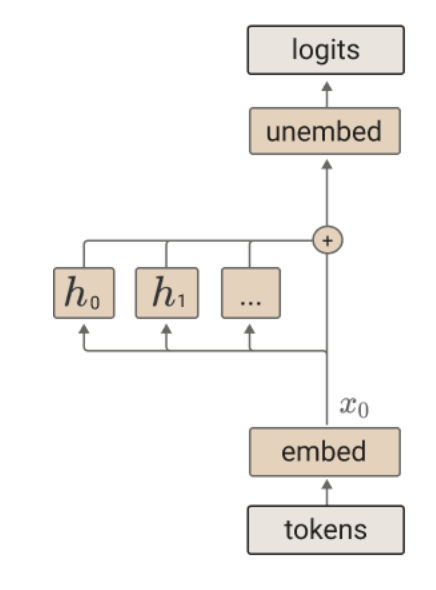
\includegraphics[height=4.6cm]{elhage.png}

      \vspace{0.05cm}
      {\muted{\footnotesize Elhage et~al.\ (2021)}\par}
    \end{column}
  \end{columns}
\end{frame}

% =====================================================================
% 24. Summary (2)
% =====================================================================
\begin{frame}{Summary}
  \vspace{-0.3cm}
  \centering
  \slidesubtitle{Vision: research taste and contribution}

  \vspace{0.5cm}
  \begin{columns}[T, totalwidth=\textwidth]
    \begin{column}{0.58\textwidth}
      \small
      \point{1}{Problems that inform probes}
        {We will work on problems whose answers inform theoretically grounded~probes.}

      \vspace{0.75cm}% match the second row of the other two-point slides
      \vspace{0.5cm}
      \point{2}{Tools we will share}
        {Our harnesses and Lean codebase will be shared with mechanistic interpretability researchers, making their own autoresearch runs easier to maintain and audit.}
    \end{column}
    \begin{column}{0.38\textwidth}
      \centering
      \vspace{0.45cm}
      
\includegraphics[width=0.62\linewidth]{vm-logo-light-bg.pdf}

      \vspace{0.3cm}
      {\muted{\footnotesize\texttt{verifiedmechanisms.ai}}\par}
    \end{column}
  \end{columns}
\end{frame}

% =====================================================================
% 25. The team
% =====================================================================
\begin{frame}{Team}
  % wording from verifiedmechanisms.ai (Team section); no names, no head counts
  \vspace{-0.3cm}
  \centering
  \slidesubtitle{Researchers in mechanistic interpretability and Lean formalisation}

  \vspace{0.5cm}
  \begin{minipage}{0.92\textwidth}
    \small
    \point{1}{Who we are}
      {An independent, grant-funded research project. The current team consists of researchers with a background in mech interp and Lean~formalisation.}

    \vspace{0.5cm}
    \point{2}{Who is joining}
      {Thanks to grantmaking.ai, more researchers will join for the next 3 months to work on the pilot project, on the \pop{mech interp} and \pop{system design} aspects.}

    \vspace{0.5cm}
    \point{3}{Supported by}
      {grantmaking.ai and BlueDot Rapid~Grant.}
  \end{minipage}
\end{frame}

% =====================================================================
% 26. To summarise
% =====================================================================
\begin{frame}{Verified Mechanisms, in pictures}
  \vspace{-0.3cm}
  \centering
  \slidesubtitle{Lowering the barriers to theoretical mech interp research.}

  \vspace{0.5cm}
  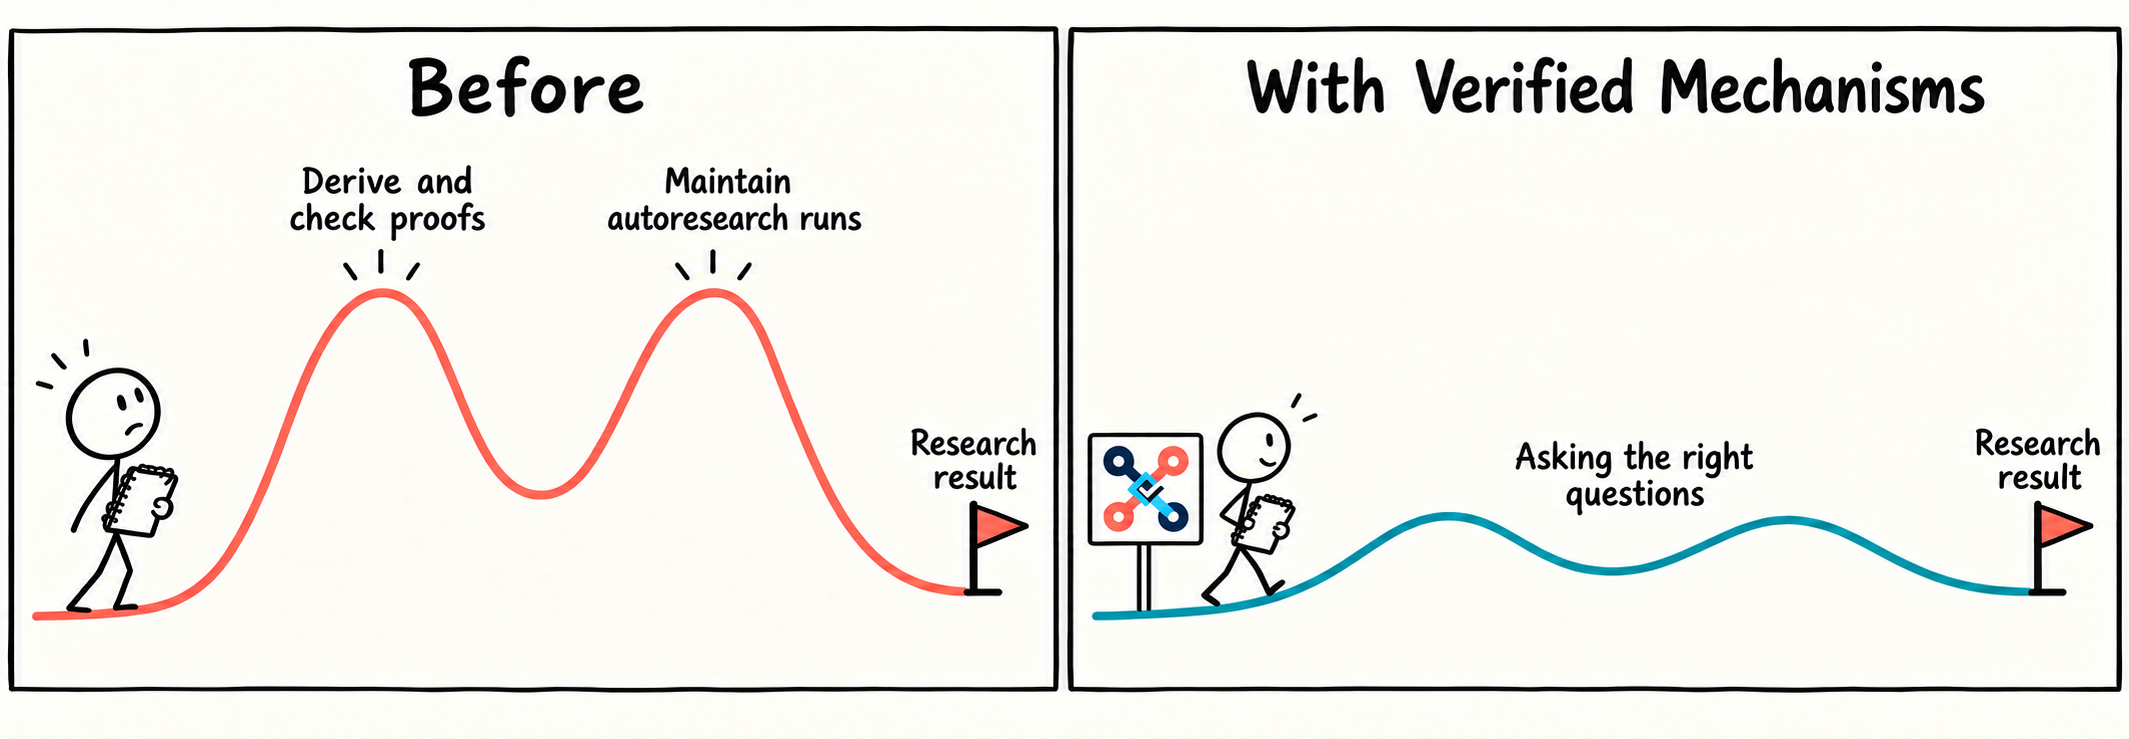
\includegraphics[width=\textwidth]{vm-comic.png}

  % \vspace{0.4cm}
  % % grant one-liner (powerful-lines.md), earmarked there as the comic caption
  % {\large\question{LLM agents do the math, Lean checks it, humans steer.}\par}
\end{frame}

% =====================================================================
% 27. Thank you
% =====================================================================
\begin{frame}[plain]
  \begin{tikzpicture}[remember picture, overlay,
      every node/.style={inner sep=0pt, outer sep=0pt}]
    \coordinate (c)  at (current page.center);
    \coordinate (sw) at (current page.south west);
    \coordinate (se) at (current page.south east);

    % thank-you block between dashed rules
    \node[anchor=center, text width=13.5cm, align=center] (ty) at ([yshift=1.15cm]c)
      {{\fontsize{30}{36}\selectfont\color{vmnavy} Thank you\par}%
       \vspace{0.3cm}%
       {\fontsize{13}{16.5}\selectfont\itshape\color{vmnavy!85}
        Questions and comments are welcome!\par}};
    \coordinate (l) at ([xshift=-5.6cm]c);
    \coordinate (r) at ([xshift=5.6cm]c);
    \coordinate (t) at ([yshift=0.5cm]ty.north);
    \coordinate (b) at ([yshift=-0.5cm]ty.south);
    \draw[vmcoral, line width=0.9pt, dash pattern=on 5pt off 3.5pt] (l |- t) -- (r |- t);
    \draw[vmcoral, line width=0.9pt, dash pattern=on 5pt off 3.5pt] (l |- b) -- (r |- b);

    % links
    \node[anchor=north, text width=13cm, align=center] at ([yshift=-0.75cm]b)
      {\muted{\small\texttt{verifiedmechanisms.ai}\quad$\cdot$\quad\texttt{github.com/VerifiedMechanisms}}\\[0.12cm]
       \muted{\footnotesize Supported by grantmaking.ai and BlueDot Rapid Grant}\par};

    % footer: VM logo (left), QR codes (centre), MATS (right), all centred on one line
    \coordinate (fl) at ([yshift=1.2cm]sw);
    \node[anchor=west] at ([xshift=1.0cm]fl)
      {
\includegraphics[height=1.3cm]{vm-logo-light-bg.pdf}};
    \node[anchor=east] at ([xshift=-1.0cm]fl -| se)
      {
\includegraphics[height=0.75cm]{mats_navy.png}};
    % QR codes, centred as a group of three
    \node[anchor=center] (q1) at ([xshift=-2.3cm]fl -| current page.center)
      {
\includegraphics[width=1.5cm]{qr-blog.png}};
    \node[anchor=north, font=\fontsize{6}{7}\selectfont, text=vmmuted] at ([yshift=-1pt]q1.south) {LW blog post};
    \node[anchor=center] (q2) at (fl -| current page.center)
      {
\includegraphics[width=1.5cm]{qr-discord.png}};
    \node[anchor=north, font=\fontsize{6}{7}\selectfont, text=vmmuted] at ([yshift=-1pt]q2.south) {Discord};
    \node[anchor=center] (q3) at ([xshift=2.3cm]fl -| current page.center)
      {
\includegraphics[width=1.5cm]{qr-xorformer.png}};
    \node[anchor=north, font=\fontsize{6}{7}\selectfont, text=vmmuted] at ([yshift=-1pt]q3.south) {GitHub};
  \end{tikzpicture}
\end{frame}

\end{document}
